\documentclass[12pt,a4paper]{article}
\usepackage[utf8]{inputenc}
\usepackage[english]{babel}
\usepackage{amsmath}
\usepackage{amsfonts}
\usepackage{amssymb}
\usepackage{makeidx}
\usepackage{graphicx}
\usepackage{lmodern}
\usepackage{kpfonts}
\usepackage{tikz}
\usepackage{hyperref}
\usepackage[left=2cm,right=2cm,top=4cm,bottom=2cm]{geometry}
\setlength{\parindent}{0px}
\author{Daniel Vázquez Lago}
\title{Propagación do son}
\begin{document}

\maketitle

\newpage

\tableofcontents

\newpage

\section{Objetivos:}
En esta práctica tenemos los siguientes objetivos:
\begin{itemize}
\item Medir la velocidad del sonido, como se comporta ante ciertos cambios, cuales son los diferentes problemas que podemos encontrar la velocidad del sonido, y como se comporta respecto al eco, en particular midiendo también la velocidad en llegar el eco al micrófono (esta última parte no realizada).  

\item Ver cuales son los modos normales en función de las condiciónes que le pongamos, ver como se comporta la onda y cuales son los problemas. 

\item Estudiar la velocidad y características en general para el modo normal con la condición de tubo cerrado. (No realizado). \\
\\
\end{itemize}

\section{Procedimiento experimental:}

\subsection{Parte 1:}

En esta parte del experimento tenemos que medir la velocidad del sonido en nuestro tubo de pitot, teniendo el tubo cerrado para evitar posibles ruidos del exterior que interfieran en el experimento (y minimizar la incertidumbre de tipo B). Para esto es muy sencillo lo que haremos: calcularemos la distancia que recorre la onda (es decir la distancia entre el altavoz y el micrófono) y lo dividiremos entre el tiempo que tarda en recorrerlo. Una buena pregunta que puede surgir en este momento es: ¿Cómo vamos a saber cuando sale la onda? Pues como la onda es producida por una pulso eléctrico que es enviado al altavoz, si conectamos el mismo aparato que produce el pulso al un osciloscopio podremos saber con muchísima precisión cuando llega la señal al altavoz (existiría un error procedente de la diferencia de llegada de estas señales, pero dada la velocidad de las cargas y lo cortos que son los cables tenerla en cuenta sería innesario, ya que es mucho menor que cualquier otro error). Además que la onda sea cuadrada nos permite distinguir con mayor exactitud cuando la onda realmente se envía. Una vez comprendido cuando sale la onda, solo nos queda distinguir cuando llega. Esto puede tener alguna complejidad, ya que el eco (que también emite un pico al llegar la onda al micrófono) y que existe bastante ruido (imposible de eliminar), pero aumentando la escala se podrá ver un pico reflejado en el osciloscopio con una diferencia temporal (mas grande cuanto mas alejado este del altavoz). Además deberíamos medir la diferencia de tiempo entre el eco y la onda enviada para contrastar también la velocidad del sonido.  

\subsection{Parte 2:} 
 
En esta parte lo que haremos es observar como se comporta la onda imponiendo diferentes condiciones de contorno, formando patrones estacionarios, que llamaremos \textit{modos normales}. Lo que haremos es estudiar las diferentes amplitudes (máximas o mínimas) para los diferentes puntos a lo largo del tubo. Además calcularemos los modos de frecuencia para los cuales hay máximos, ya que para ciertas frecuencias no hay máximos ni mínimos de amplitud (o son muy pequeños). Esto se debe a que al imponer ciertas condiciones de contorno realmente lo que estamos haciendo es crear una interferencia entre ondas las cuales pueden ser constructivas (los casos que estudiamos) o destructivas (casos en los que no se escucharía nada en ningún sitio del tubo). Gracias a esto comprobaremos cuales son los patrones de frecuencia, y verificar una función que nos permita saber cuando ocurren estas interferencias constructivas. Además de estudiarlo de manera esquemática debemos estudiarlo de manera mas precisa en el caso del tubo cerrado (calculando las amplitudes). 
 
\section{Análisis de datos:}

\subsection{Parte 1: \label{SS:parte 1}}
Como ya dijimos en esta parte nos centraremos en el cálculo de la velocidad del sonido. Para eso obtuvimos los datos:  \\


De los cuales podemos extraer una regresión lineal con los siguientes resultados: \\

\begin{figure}[h!] \centering 
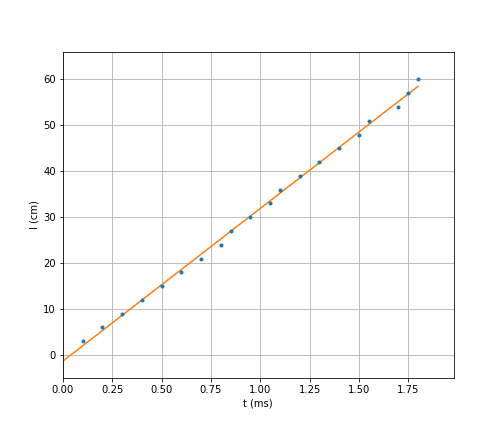
\includegraphics[scale=0.6]{regresiónlineal.png}
\caption{distancia del micrófono (cm) frente distancia temporal de la onda (ms)}
\label{fig:velocidad-sonido}
\end{figure}

\begin{table}[h!]
\centering
\begin{tabular}{|c|c|c|c|c|}
\hline
a  (cm)	 & s(a) (cm) 	 & b (dam/s)	 & s(b) (dam/s) 	 & r \\   \hline
-1.319 	 & 0.096 	 & 33.234 	 & 0.086 	 & 0.9996 \\ \hline
\end{tabular}
\caption{tabla de datos de la regresión lineal}
\label{tab:velocidad-sonido}
\end{table}

De lo que podemos extraer que b es la velocidad del sonido. Haciendo el cambio de escala tendríamos que:

$$ v = 332,34 \pm 0.86  \ m/s$$

Sin embargo: ¿Qué es a?. Pues como se puede ver a tiene dimensiones de distancia, con lo cual tiene que estar relacionado con nuestro tubo de pitot, o con las medidas tomadas de distancia. Podríamos tomarlo como un error sistemático dado al tomar las distancias (ya que sería presentado por todos y cada uno de los datos). Cuando realizamos el experimento nos podemos dar cuenta de que el altavoz está a una distancia del comienzo de la regla entre 1 o 2 cm: ¡Qué es precisamente el valor de a!. Sin embargo también puede tener otra naturaleza añadida (aunque con mucho menos "fuerza" que la anterior). Aunque nosotros veamos con cierta precisión donde está el micrófono, realmente no sabemos si el detector está justamente donde marcamos (quizás esté mas atrás). Aún así esta diferencia no debe ser mas de unos pocos milímetros, pero podríamos tenerla en cuenta. Es negativo porque realmente el altavoz está "ubicado" en -1.3 cm. \\


Ahora vendría la parte de calcular el eco, contrastar el resultado anterior (y ver que realmente si que se verfica). Por desgracia no fue realizada, dado la falta de tiempo para realizar la práctica. Sin embargo, aunque no esté acabada, si que pudimos observar que el eco existe y que a mas distancia respecto al altavoz hay dos "perturbaciones" observables en el osciloscopio que cada vez se van juntando mas llegando a ser prácticamente indistinguibles cuando l =  60 cm (que es donde el tubo esta cerrado). De hecho uno de los grandes puntos de la práctica es ser capaz de distinguir la perturbación producida por el sonido y por el eco, aunque se puede diferenciar simplemente cogiendo el micrófono y moviéndolo. Como podemos intuir, si la perturbación a medida que acercamos el micrófono se desplaza hacia la derecha por el osciloscopio, acercándose cada vez mas a la perturbación del altavoz, estamos ante la perturbación del sonido. Si se aleja cada vez más, a la del eco. 

\subsection{Parte 2:}
Como dijimos en esta parte estudiamos los diversos modos normales dadas diferentes condiciones de contorno. Reflejaremos en las siguientes gráficas cuales son (de manera esquemática, no pretenden ser un esquema totalmente real). \\

Tubo abierto: \\

\begin{center}
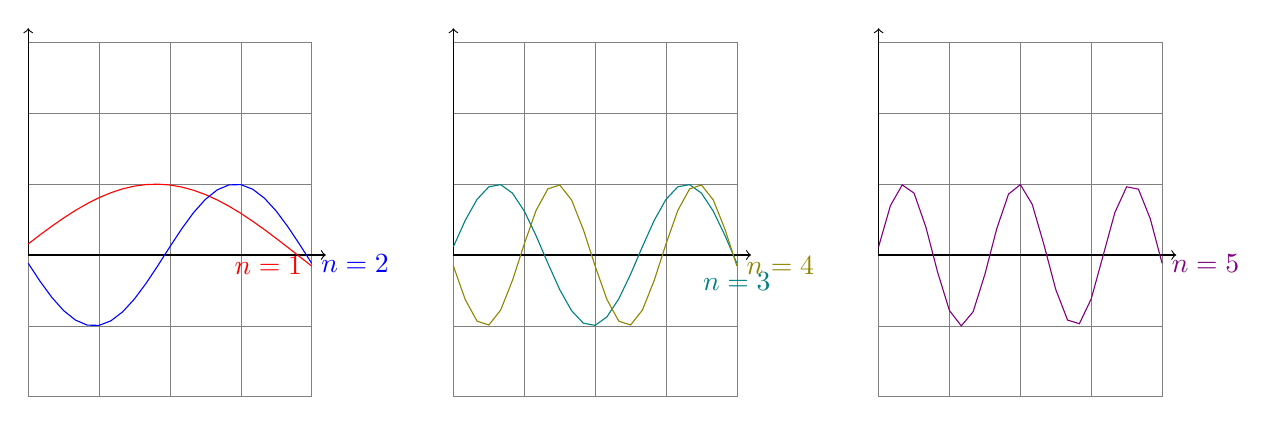
\begin{tikzpicture}[xscale=0.9, yscale=0.9] \centering
\draw[very thin,color=gray] (0,-2) grid (4,3);
\draw [<->] (0,3.2)-- (0,0)-- (4.2,0); 
\draw [red,domain=0.2:4.2] plot (\x-0.2, {sin(\x*pi/4r)})
	node[left] {$n=1$}; 
\draw [blue,domain=0.075:4.075] plot (\x-0.075, -{sin(\x*pi*4/8 r)})
	node[right] {$n=2$}; 
	

\draw[very thin,color=gray] (6,-2) grid (10,3);
\draw [<->] (6,3.2)-- (6,0)-- (10.2,0);
\draw [teal,domain=6.05:10.05] plot (\x-0.05, {sin(\x*pi*6/8 r-6*pi*6/8 r)})
	node[below] {$n=3$}; 
\draw [olive,domain=6.05:10.05] plot (\x-0.05, -{sin(\x*pi*8/8 r - 6*pi*8/8 r)})
	node[right] {$n=4$};

\draw[very thin,color=gray] (12,-2) grid (16,3);
\draw [<->] (12,3.2)-- (12,0)-- (16.2,0);
\draw [violet,domain=12.03:16.03] plot (\x-0.03, {sin(\x*pi*10/8 r-12*pi*10/8 r)}) 
node[right] {$n=5$}; 
\end{tikzpicture}
\end{center}

Tubo semiabierto:

\begin{center}
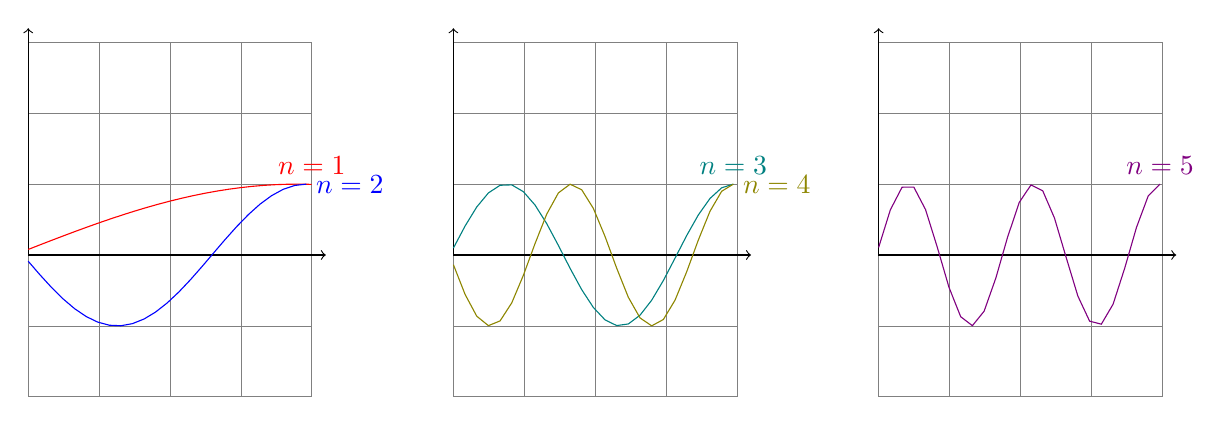
\begin{tikzpicture}[xscale=0.9, yscale=0.9] 
\draw[very thin,color=gray] (0,-2) grid (4,3);
\draw [<->] (0,3.2)-- (0,0)-- (4.2,0); 
\draw [red,domain=0.2:4.2] plot (\x-0.2, {sin(\x*pi/8r)})
	node[above] {$n=1$}; 
\draw [blue,domain=0.075:4] plot (\x-0.075, -{sin(\x*pi*3/8 r)})
	node[right] {$n=2$}; 
	

\draw[very thin,color=gray] (6,-2) grid (10,3);
\draw [<->] (6,3.2)-- (6,0)-- (10.2,0);
\draw [teal,domain=6.05:10] plot (\x-0.05, {sin(\x*pi*5/8 r-6*pi*5/8 r)})
	node[above] {$n=3$}; 
\draw [olive,domain=6.05:10] plot (\x-0.05, -{sin(\x*pi*7/8 r - 6*pi*7/8 r)})
	node[right] {$n=4$}; 
	


\draw[very thin,color=gray] (12,-2) grid (16,3);
\draw [<->] (12,3.2)-- (12,0)-- (16.2,0);
\draw [violet,domain=12.03:16] plot (\x-0.03, {sin(\x*pi*9/8 r-12*pi*9/8 r)}) 
node[above] {$n=5$}; 
\end{tikzpicture}
\end{center}

Se puede ver perfectamente que el modo abierto no acaba ni empieza en el nodo. Esto se debe a que realmente el micrófono no está colocado en el punto del nodo perfectamente, ya que es muy dificil ubicarlo en esa posición (justo delante del altvoz, justo donde está abierto). De todos modos insto que esto no es una representación fidedigna, simplemente una esquematización de lo que observamos. \\ 

Como tenemos la frecuencia para cada modo y la velocidad del sonido (obtenido en la subsección \ref{SS:parte 1}), podemos aplicar la siguiente fórmula para obtener la longitud de onda para cada modo normal (y su incertidumbre): 

\begin{equation}
\nu_n \lambda_n = v_{sonido}
\end{equation}

Podemos ver los datos en la siguientes tablas:

\begin{table}[h!] \centering
\begin{tabular}{|c|c|c|c|c|}
\hline  modo 	 & $f_i \ (Hz)$ 	 &  $s(f_i) \ (Hz) $ 	 & $\lambda_i \ (m)$ 	 & $s(\lambda_i) \ (m)$  \\ \hline 
1 	 & 185 	 & 13	 & 1.79 & 0.13  \\ 
2 	 & 416	 & 69	 & 0.80 	 & 0.13  \\ 
3 	 & 714	 & 51	 & 0.47 	 & 0.033  \\ 
4 	 & 1000	 & 100 	 & 0.33 	 & 0.033  \\ 
5 	 & 1250	 & 156	 & 0.27 	 & 0.033  \\  \hline 
\end{tabular}
\caption{valores de f y $\lambda$ para los modos normales del tubo semi-abierto}
\end{table}

\begin{table}[h!] \centering
\begin{tabular}{|c|c|c|c|c|} \hline 
modo 	 & $f_i \ (Hz)$ 	 &  $s(f_i) \ (Hz) $ 	 & $\lambda_i \ (m)$ 	 & $s( \lambda_i ) \ (m) $  \\ \hline 
1 	 & 217.4 	 & 9.5 	 & 1.529	 & 0.067  \\ 
 2 	 & 400	 & 16	 & 0.83 	 & 0.033 \\ 
 3 	 & 625	 & 39 	 & 0.53	 & 0.033  \\ 
 4 	 & 833   & 69 	 & 0.40 	 & 0.033  \\ 
 5 	 & 1052 	 & 111 	 & 0.32 	 & 0.033  \\  \hline
\end{tabular}
\caption{valores de f y $\lambda$ para los modos normales del tubo abierto}
\end{table}
Ahora podemos obtener el valor de la función f(n) (ya que conocemos L) para los modos normales, ya que:

\begin{equation}
L = f(n) \dfrac{\lambda_n}{4} \label{Ec:función-n}
\end{equation}

Entonces los valores de f(n) para los modos normales del tubo semi-abierto:  \\

\begin{table}[h!]\centering
\begin{tabular}{|c|c|c|c|c|}
\hline  
 $f(1)$ 	 & $f(2)$ 	 & $f(3)$ 	 & $f(4)$ 	 & $f(5)$ \\ \hline 
1.337320 	 & 3.008970 	 & 5.158234 	 & 7.221527 	 & 9.026909 	 \\
 \hline 
\end{tabular}
\caption{valores de f(n) para tubo semi-abierto}
\end{table}

Del tubo abierto: 
\begin{table}[h!]\centering
\begin{tabular}{|c|c|c|c|c|}
\hline  
 $f(1)$ 	 & $f(2)$ 	 & $f(3)$ 	 & $f(4)$ 	 & $f(5)$ \\ \hline 
2.093196 	 & 3.851481 	 & 6.017939 	 & 8.023919 	 & 10.135476 \\
 \hline 
\end{tabular}
\caption{valores de f(n) para tubo abierto}
\end{table}



Si nos damos cuenta podemos ver que f(n) se comporta de una manera sumamente parecida a la siguiente función para el tubo semi-abierto:  

\begin{equation}
f(n) = 2n-1
\end{equation}

Para el tubo semiabierto: 

\begin{equation}
f(n) = 2n
\end{equation}

Cuadra perfectamente con las funciones que estudiamos en fisica II. Es decir que lo que hemos estudiado teóricamente cuadra con lo demostrado experimentalmente. De la ecuación \ref{Ec:función-n} se puede extraer que:

\begin{equation}
\dfrac{\nu_n}{\nu_m} = \dfrac{f_n}{f_m}
\label{eq:funciones}
\end{equation}

Que comprobaremos para el caso semi-abierto (consideramos el caso n=m=1 trivial):
$$ \dfrac{\nu_2}{\nu_1}=2.25, \ \dfrac{f(2)}{f(1)}=2.24 ; \quad \dfrac{\nu_3}{\nu_1}=3.86  \ \dfrac{f(3)}{f(1)}=3.85 \ldots $$
No calculamos mas datos porque los que se muestran son suficientemente significativos. Son prácticamente indénticos, probablemente si tuviéramos en cuenta mas decimales serían iguales. Para el caso abierto:
$$ \dfrac{\nu_2}{\nu_1}=1.84, \ \dfrac{f(2)}{f(1)}=1.84 ; \quad \dfrac{\nu_3}{\nu_1}=2.87  \ \dfrac{f(3)}{f(1)}=2.88 \ldots$$
Son igual de parecidos que el caso anterior. Por lo tanto queda demostrada la ecuación \ref{eq:funciones}.

\section{Conclusión}
Como podemos ver todos los datos han salido como queríamos: la velocidad del sonido es muy similar a la real (tan solo difieren en 7 m/s), que se puede deber a la diferencia de condiciones ambientales (temperatura, presión, humedad...) como a factores humanos (ruido, vibraciones en la mesa...) e instrumentales (falta de precisión de los aparatos, mala calibración)... De todos modos son unos datos muy buenos, y mas si nos fijamos en el coeficiente de regresión lineal. \\

En la segunda parte también, las funciones cuadran perfectamente con lo que estudiamos teóricamente, así como con lo que queremos demostrar. De hecho, tal y como hemos deducido f(n) para el caso semi-abierto y abierto podremos deducirlo para el caso cerrado:

\begin{equation}
f(n) = 2n 
\end{equation}

Se comporta igual que el caso abierto pero en este caso en vez de tener dos nodos tiene dos máximos. La única diferencia sería cambiar la ecuación sinuidal a cosenuidal, es decir, cambiar de fase en $\pi/2$. \\

 %Otra de las grandes preguntas que nos podemos hacer es que por qué cambia la amplitud de signo al pasar por un nodo. La explicación física es bien sencilla: la longitud del tubo no cambia al aplicarle una onda, pero la onda si cambia las partículas de dentro, haciendo que se desplacen hacia un punto de densidad máximo (anti-nodo) tiene que existir. \\
 
Con esto damos concluida la práctica de propagación del sonido, muy satisfechos con los resultados.  

\section{Comentarios adicionales}
\begin{itemize}
\item Debido a la falta de tiempo y la ausencia de mi compañero no pude realizar dos partes de la práctica. 
\item No se pusieron los datos tomados experimentalmente (como el periodo, las incertidumbres del periodo, las distancias o los tiempos de la parte 1). 
\end{itemize}
\end{document}